\subsection{Sequence Diagram}

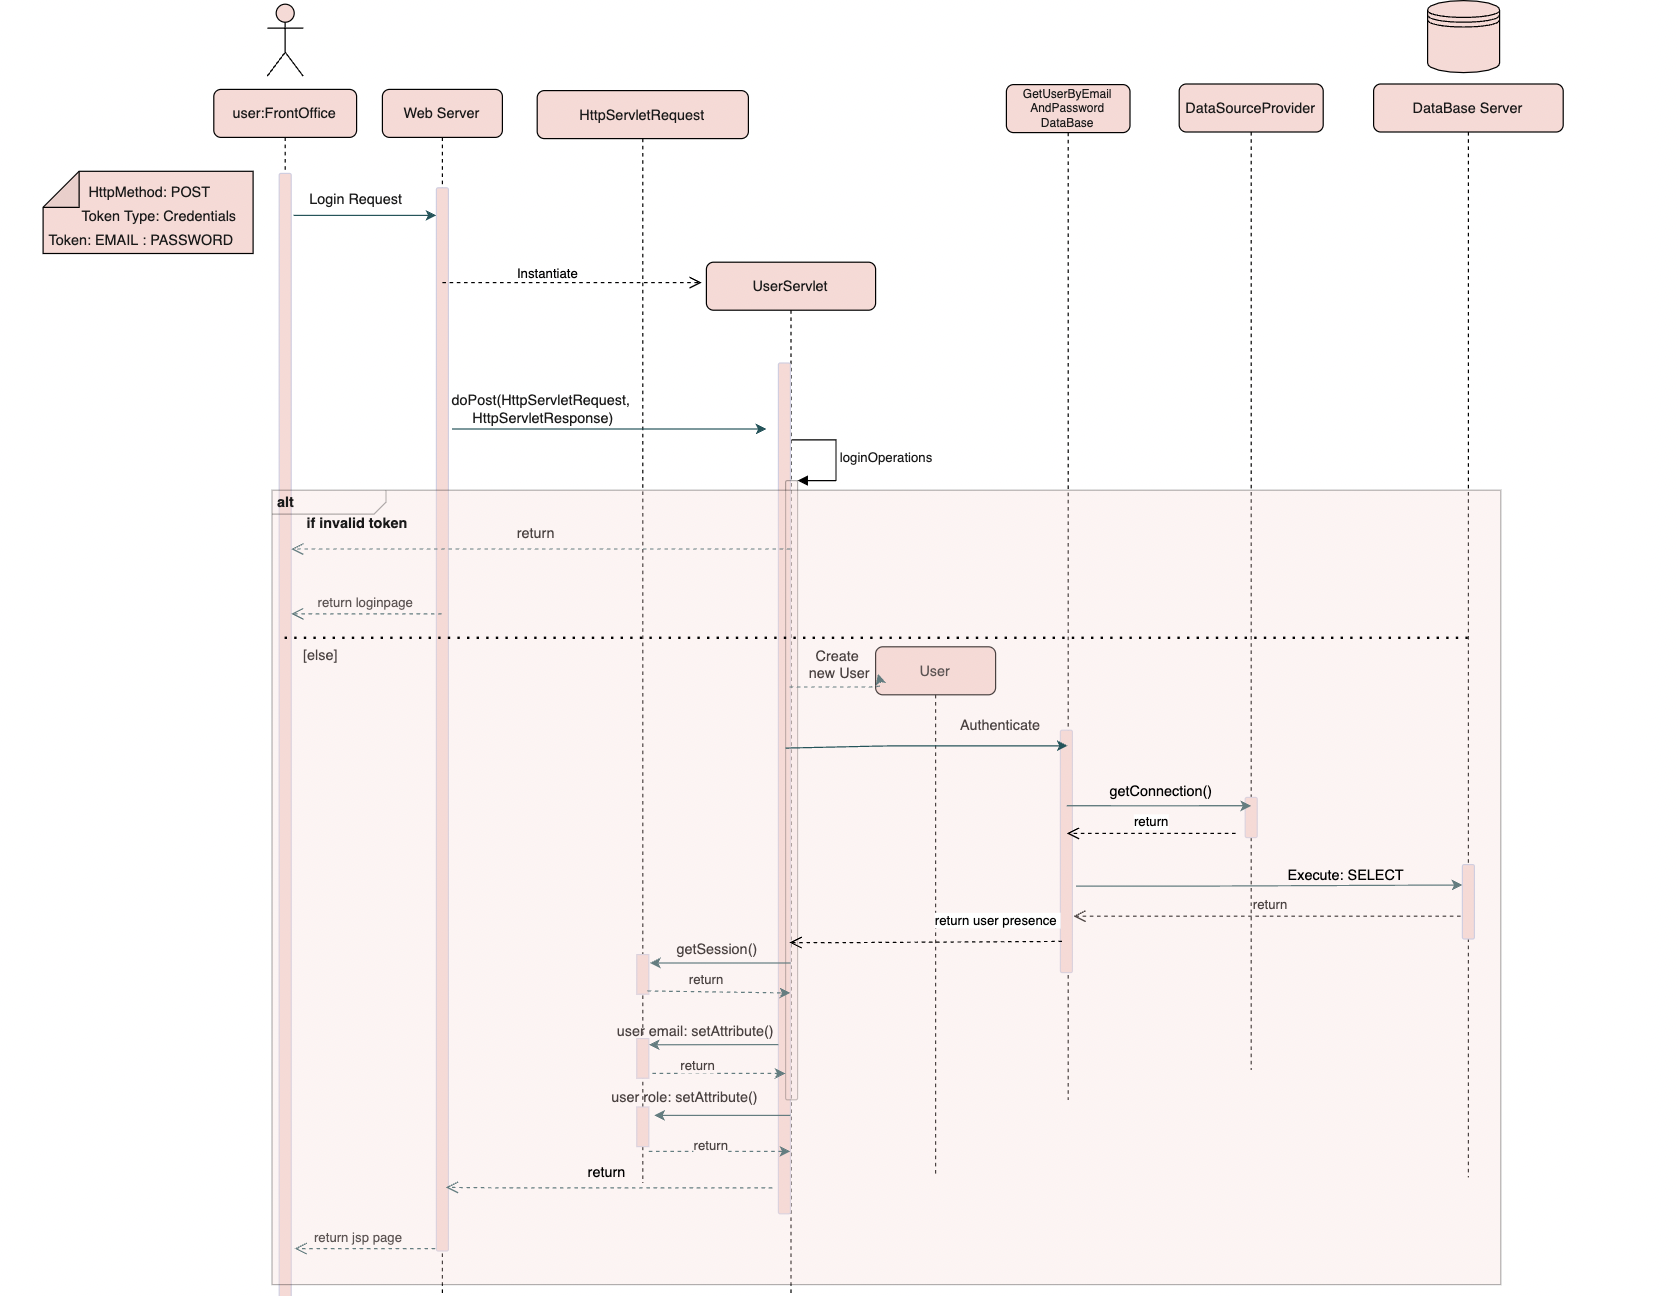
\includegraphics[width=\textwidth]{images/SequenceDiagram_LoginUser.png}

The sequence diagram illustrates the login operations for the front office user in the application. A 
Login Request is sent from the user to the web server in by the HTTPMethod POST and simultaneously  passing the applied email and password credentials. Further on, the web server instantiates the UserServlet and calls the doPost Method which passes the HttpServletRequest and HttpServletResponse. After recognizing the request as an attempt to login the UserServlet calls the method loginOperations to verify the given credentials. If credentials are invalid or missing, it returns the login jsp-file with the attached error message, and else a new user object is initialized with its data. The new user object data needs to be authenticated and is being passed on as an argument to the method responsible. The method in the DAO-class (GetUserByMailAndPasswordDatabase) requests a connection to the DataSourceProvider. This makes it possible for the DAO-class to retrieve information about whether the given user is current in the database or not from the database server. The information is then being returned to the UserServlet. After retrieving the session with the users email and role as parameters from HttpServletRequest, the user is being forwarded to the instantiated homepage.jsp  with the user´s data. 

%\includegraphics[width=\columnwidth]{images/sequenceDiagram.pdf}
%describe here the sequence diagram